% A simple graph with straight and bend arrows and loops
% Stefan Kottwitz
\documentclass{article}
\usepackage{tikz}
\usetikzlibrary{arrows}
\begin{document}
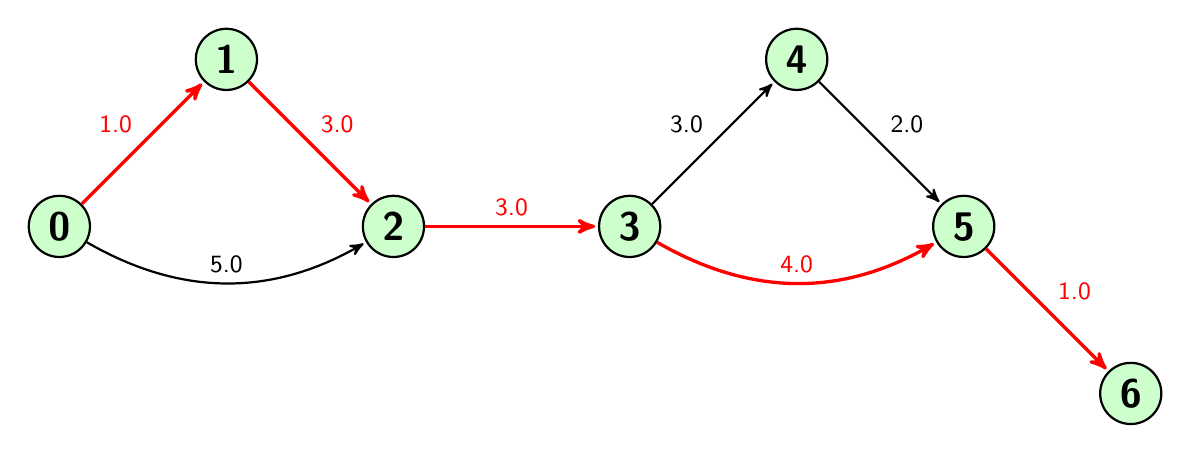
\begin{tikzpicture}[->,>=stealth',shorten >= 1pt,auto,node distance=3cm,
  thick,main node/.style={circle,fill=green!20,draw,font=\sffamily\Large\bfseries}]

  \node[main node] (0) {0};
  \node[main node] (1) [above right of=0] {1};
  \node[main node] (2) [below right of=1] {2};
  \node[main node] (3) [	  right of=2] {3};
  \node[main node] (4) [above right of=3] {4};
  \node[main node] (5) [below right of=4] {5};
  \node[main node] (6) [below right of=5] {6};

  \path[every node/.style={font=\sffamily\small}]
    (0) edge [red, very thick] node [auto]  {1.0} (1)
    	edge [bend right] node [auto] {5.0} (2)
    (1) edge [red, very thick] node [auto] {3.0} (2)
    (2) edge [red, very thick] node [auto] {3.0} (3)
    (3) edge node [auto] {3.0} (4)
    	edge [bend right, red, very thick] node [auto] {4.0} (5)
    (4) edge node [auto] {2.0} (5)
    (5) edge [red, very thick] node [auto] {1.0} (6);

\end{tikzpicture}
\end{document}